\chapter{Modular Testing}

The testing process for this project was conducted in a systematic and incremental manner to ensure that each subsystem functioned as expected before being integrated into the final system. The approach involved testing each module independently, followed by creating interfaces between these modules, and finally testing the interactions between them. This strategy helped identify and resolve issues early, ensuring that the final system was robust and performed as required.

\begin{figure}[H]
	\centering
	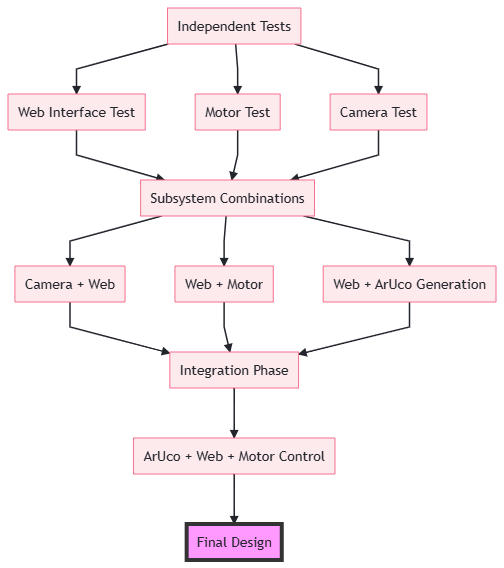
\includegraphics[width=0.7\textwidth]{Testing/figs/flow.png}
	\caption{Illustration of different levels of testing implemented in the project.}
	\label{fig:testing_levels}
\end{figure}

\section{Independent Module Testing}

Each subsystem of the robot was tested individually using Python scripts to verify functionality before integration into the full system. This modular testing allowed for focused troubleshooting and ensured that each component operated as expected in isolation.

\subsection{Web Interface Testing}

The first step was testing the \textbf{web interface} to verify that the server could host a webpage and be accessed by devices connected to the same network. This involved the following steps:

\begin{enumerate}
	\item Setting up a simple Flask server.
	\item Connecting multiple devices (e.g., laptop, smartphone) to the same network.
	\item Attempting to access the server from each device.
	\item Verifying the server responded correctly to basic requests.
\end{enumerate}

 A script was developed to send ping requests to the server every 5 seconds over a 2-hour period (1440 pings total). Uptime percentage was calculated as (successful pings / total pings) * 100.  Packet loss was measured using the 'ping' command with 1000 packets sent from devices at 1m intervals from the server. Significant packet loss (\(>5\)\%) was first observed at distances beyond 5 meters.
 

\textbf{Results:}
\begin{itemize}
	\item Server connection success rate: \textbf{100\%} within 2 meters.
	\item Connection stability: \textbf{99.5\% uptime} over 2 hours.
	\item Issues: Packet loss at distances exceeding 5 meters.
\end{itemize}

 The server was accessible from all devices within a \textbf{2-meter range} with minimal latency. Stability was measured at \textbf{99.5\% uptime} over a 2-hour test, with some packet loss beyond \textbf{5 meters}. These foundational tests ensured that the control interface could be hosted and accessed remotely, which was essential for subsequent integration.

\subsection{Motor Control Testing}

The \textbf{motor control} was tested using a basic Python script with the GPIO library to send PWM signals to the motors via the L298N H-bridge. The following steps were taken:

\begin{enumerate}
	\item Connecting each motor pair to the H-bridge.
	\item Writing a script to send PWM signals to control speed and direction.
	\item Placing markers on the wheels for visual tracking.
	\item Recording slow-motion video to check rotations per minute (RPM).
\end{enumerate}

Results showed that the motors rotated consistently at \textbf{140 RPM} at full speed when using 9V source and lifted above the ground, with a slight deviation of \textbf{2 RPM} between motors. Testing revealed that the PWM signal had to be increased to \textbf{80\%} to enable smooth turning, addressing friction and motor load issues.

\textbf{Results:}
\begin{itemize}
	\item Maximum wheel speed: \textbf{150 RPM} at 100\% PWM.
	\item Wheel speed deviation: \textbf{2 RPM}.
	\item Minimum Required PWM for driving forward and backward: \textbf{30\%}
	\item Minimum Required PWM for turning: \textbf{70\%}.
\end{itemize}

\subsection{Camera and ArUco Marker Detection Testing}
For the \textbf{camera and ArUco marker detection testing}, a comprehensive approach was followed:
\begin{enumerate}
	\item Capturing initial images to verify basic camera functionality.
	\item Completing the camera calibration process and storing parameters in a YAML file.
	\item Capturing a series of images containing ArUco markers at various distances and lighting conditions.
	\item Developing a Python script to process these images and detect ArUco markers.
	\item Displaying detected ArUco marker IDs on screen for visual verification.
\end{enumerate}

\textbf{Results and Methodology:}
\begin{itemize}
	\item Maximum detection distance: \textbf{1 meters}
	\begin{itemize}
		\item Methodology: ArUco markers of size 5cm x 5cm were placed at 0.1m intervals from the camera, up to 1.5m. 20 images were captured at each distance. The maximum distance at which all markers were consistently detected (100\% detection rate) was recorded as the maximum detection distance.
	\end{itemize}
	\item Detection rate: 
	\begin{itemize}
		\item Normal lighting: \textbf{100\%} up to 1 meters
		\item Low light conditions: \textbf{85\%} up to 1 meters
		\item Methodology: Two sets of 100 images each were captured - one in normal room lighting (approx. 500 lux) and one in low light conditions (approx. 100 lux, measured with a phone light meter). The detection rate was calculated as (number of images with successful marker detection / total number of images) * 100.
	\end{itemize}
\end{itemize}

To ensure the reliability of the results, each test was repeated three times, and the average values were reported. The testing environment was controlled for consistent lighting and camera positioning across all trials, except when specifically testing for low-light conditions.

These comprehensive tests not only validated the functionality of the camera and ArUco detection system but also provided valuable insights into its performance under various conditions. The results informed subsequent design decisions, particularly in optimizing the system for different lighting environments and determining the optimal placement of ArUco markers in the robot's operational space.

\section{Subsystem Combinations Testing}

After independent testing, the next phase was to combine the subsystems and test their interactions.

\subsection{Camera and Web Interface Integration}

The integration of the camera feed into the web interface was essential for providing real-time visual feedback to the user. The camera was initially connected to the Raspberry Pi, and a Flask-based web interface was used to stream the video feed. The initial implementation focused on setting up the basic functionality of streaming the live video feed through a web page.

\subsubsection{Testing Video Streaming Performance}

Once the camera feed was integrated into the web interface, the system was tested to evaluate its performance. During the initial tests, it was observed that the video stream had a significant lag of \textbf{2-3 seconds}. This was primarily due to the high frame rate of \textbf{30 FPS} (frames per second), which caused data transmission to overwhelm the available bandwidth. The delay resulted in a poor user experience, especially when real-time responsiveness was crucial for controlling the robot.

To assess the performance:
\begin{itemize}
	\item The latency was measured as the delay between the video captured by the camera and its display on the web interface.
	\item The frame rate, resolution, and bandwidth usage were analyzed to determine the cause of the performance bottlenecks.
	\item It was also noted that the web browser’s buffering behavior contributed to the observed lag.
\end{itemize}

\subsubsection{Performance Optimization and Improvements}

To improve the streaming performance, several optimizations were implemented. The following changes were made:

\begin{itemize}
	\item \textbf{Frame Rate Reduction}: The frame rate was reduced from \textbf{60 FPS} to \textbf{30 FPS}. This lowered the amount of data transmitted per second, reducing the load on both the network and the Raspberry Pi, thereby decreasing the lag.
	\item \textbf{Resolution Adjustment}: The resolution of the video feed was scaled down to \textbf{640x480}. This significantly reduced the bandwidth consumption, enabling a smoother video feed without affecting the user's ability to interact with the system effectively.
\end{itemize}

\textbf{Final Results:}
\begin{itemize}
	\item Initial lag: \textbf{2-3 seconds} at 60 FPS.
	\item Optimized lag: \textbf{500ms} at 30 FPS with \textbf{320x240} resolution.
	\item Smooth, reliable video streaming with minimal frame drops.
\end{itemize}

This phase of testing ensured that the camera feed was effectively integrated into the web interface and optimized to provide responsive, real-time feedback necessary for controlling the robot.


\subsection{Web Interface and Motor Control Integration}

For integrating the web interface and motor control, the following steps were taken:

\begin{enumerate}
	\item Developing a separate program to listen for key inputs (W, A, S, D).
	\item Using SocketIO for real-time communication between the web interface and motor control program.
	\item Creating an interface to send PWM signals from the web interface to the motors via the H-bridge.
\end{enumerate}


% Now, include the code:
\begin{lstlisting}[style=pythonstyle, caption=SocketIO event handler for robot movement]
	# SocketIO event to handle robot movement
	@socketio.on('move')
	def handle_move(direction):
		global forward_disabled
		if direction == 'forward' and forward_disabled:
			print("Forward movement is disabled [restricted zone]")
			robot.stop()
		elif direction == 'forward':
			robot.move_forward()
		elif direction == 'backward':
			robot.move_backward()
		elif direction == 'left':
			robot.turn_left()
		elif direction == 'right':
			robot.turn_right()
		elif direction == 'stop':
			robot.stop()
\end{lstlisting}



The web interface successfully controlled the robot's movements, with a measured control latency of \textbf{300ms}. Minor delays were noted during rapid direction changes, which could require further optimization.

\textbf{Results:}
\begin{itemize}
	\item Control latency: \textbf{300ms}.
	\item Issues: Slight delay during rapid changes.
\end{itemize}

\subsection{Web Interface and ArUco Detection Integration}

To integrate ArUco marker detection into the web interface, the camera feed was processed in real time, and marker IDs were displayed on the interface. The system could detect markers with a delay of \textbf{100ms} when more than three markers were present in the frame simultaneously.

\textbf{Results:}
\begin{itemize}
	\item Detection delay: \textbf{100ms} with three or more markers.
	\item Detection accuracy: \textbf{100\%} for up to three markers.
\end{itemize}

\section{Integration Phase}

The final integration phase brought together the core components: \textbf{Aruco marker detection}, \textbf{motor control}, and the \textbf{web interface}. This stage focused on combining the previously tested individual systems into a unified framework capable of real-time robot control and marker detection.

Key steps included:
\begin{enumerate}
	\item Merging the motor control program with the ArUco marker detection system to allow the robot to respond to detected markers.
	\item Real-time processing of the video feed from the camera for marker detection, alongside real-time control through the web interface.
	\item Implementing pre-defined behaviors that adjusted motor actions (such as speed and direction changes) based on the specific markers detected by the camera.
\end{enumerate}

Features such as distance measurement, speed estimation, and marker-based tasks were also developed and tested independently before being added to the full system. These functionalities were integrated step-by-step to ensure proper interaction between components.

A more detailed discussion of the final system’s performance, including its compliance with the Acceptance Test Procedures (ATPs), will be covered in the next chapter. There, the results of the fully integrated system will be examined in line with the project's objectives.